\section{Hybrid version analysis}

Figure \ref{fig:plot-hybrid-int} shows a comparison between the vanilla and the hybrid version on both inputs. We tested different hybrid configurations and grain sizes. First, we can observe both cases that hybridizing does not add overheads. We can compare the \textit{48x1} and the \textit{48x0} configurations and see that the time is nearly equal excepting the reduced case with grain size one that the number of tasks is high and increments the execution time notably. In general terms, hybridization improves the integration time because OmpSs allows improving the load balance among threads. On the detailed case (Figure \ref{fig:plot-hybrid-int-det}) we perceive that the grain size does not impact the performance, although we identify the value 32 as the ideal. The best hybrid configuration for the detailed case is \textit{6x8}. On the reduced case (Figure \ref{fig:plot-hybrid-int-red}) we observe grain size affects the performance. Low grainsize values make the number of tasks increase which adds overhead from making the runtime process tasks. The grainsize values that best fit is greater than 4. The ideal hybrid configuration is \textit{4x12}.

\begin{figure}[ht]
  \begin{subfigure}{1\textwidth}
    \centering
    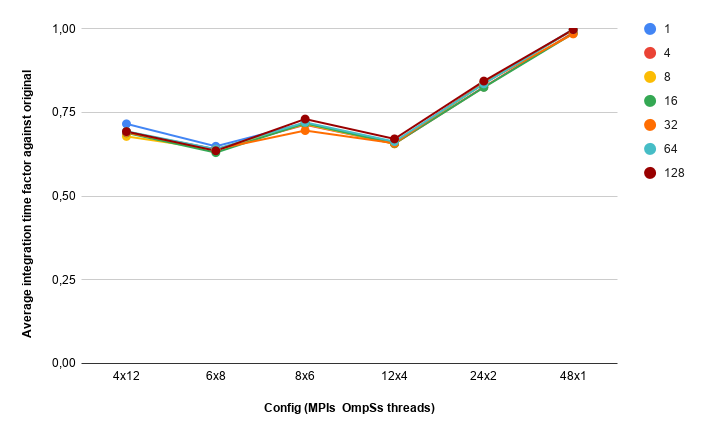
\includegraphics[width=0.7\textwidth]{graphics/hybridcomplete.png}
    \subcaption{Detailed chemistry case}
    \label{fig:plot-hybrid-int-det}

  \end{subfigure}
  \begin{subfigure}{1\textwidth}
    \centering
    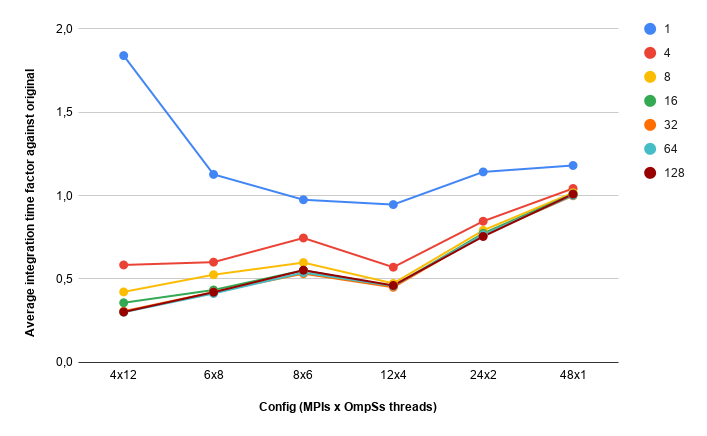
\includegraphics[width=0.7\textwidth]{graphics/hybridreduced.png}
    \subcaption{Reduced chemistry case}
    \label{fig:plot-hybrid-int-red}

  \end{subfigure}

  \caption[Hybrid chemical integration timing comparison.]{Hybrid chemical integration timing comparison. Own compilation.}
  \label{fig:plot-hybrid-int}
\end{figure}

Although hybridization improves the integration time sustainably, the application performance is diminished. 
Figure \ref{fig:plot-hybrid-int-it} shows the same plot but comparing against the iteration time. We can observe that hybridization reduces overall performance. The whole application not being hybridized causes an inefficient usage of the resources and adds unnecessary overheads. This fact makes that we decide to use \textit{48x1} version in both cases as the best for adding DLB. The negative impact of hybridization is higher on the reduced chemistry (Figure \ref{fig:plot-hybrid-int-red-it}) as the integration time weight is lower.

\begin{figure}[ht]
  \begin{subfigure}{1\textwidth}
    \centering
    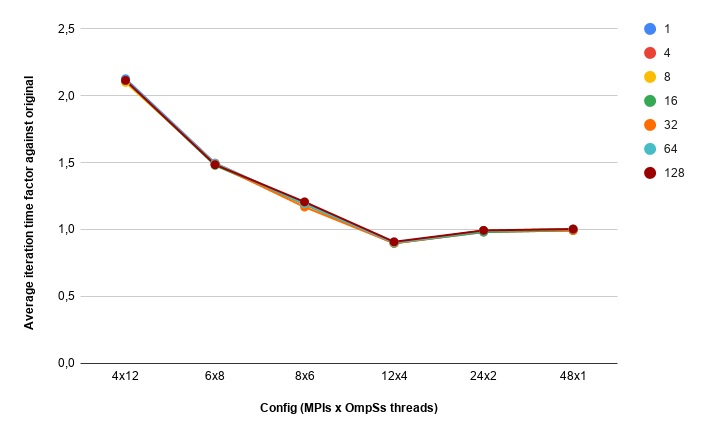
\includegraphics[width=0.7\textwidth]{graphics/hybridcompleteabs.png}
    \subcaption{Detailed chemistry case}

  \end{subfigure}
  \begin{subfigure}{1\textwidth}
    \centering
    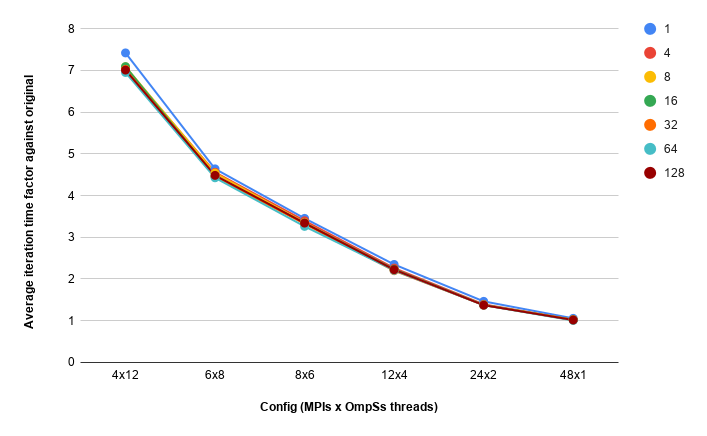
\includegraphics[width=0.7\textwidth]{graphics/hybridreducedabs.png}
    \subcaption{Reduced chemistry case}
    \label{fig:plot-hybrid-int-red-it}

  \end{subfigure}

  \caption[Hybrid iteration timing comparison.]{Hybrid iteration timing comparison. Own compilation.}
  \label{fig:plot-hybrid-int-it}
\end{figure}


